%!TEX root = gorila_paper.tex
\section{Distributed Architecture}

\begin{figure*}[ht]
	%\vskip 0.2in
	\begin{center}
		\centerline{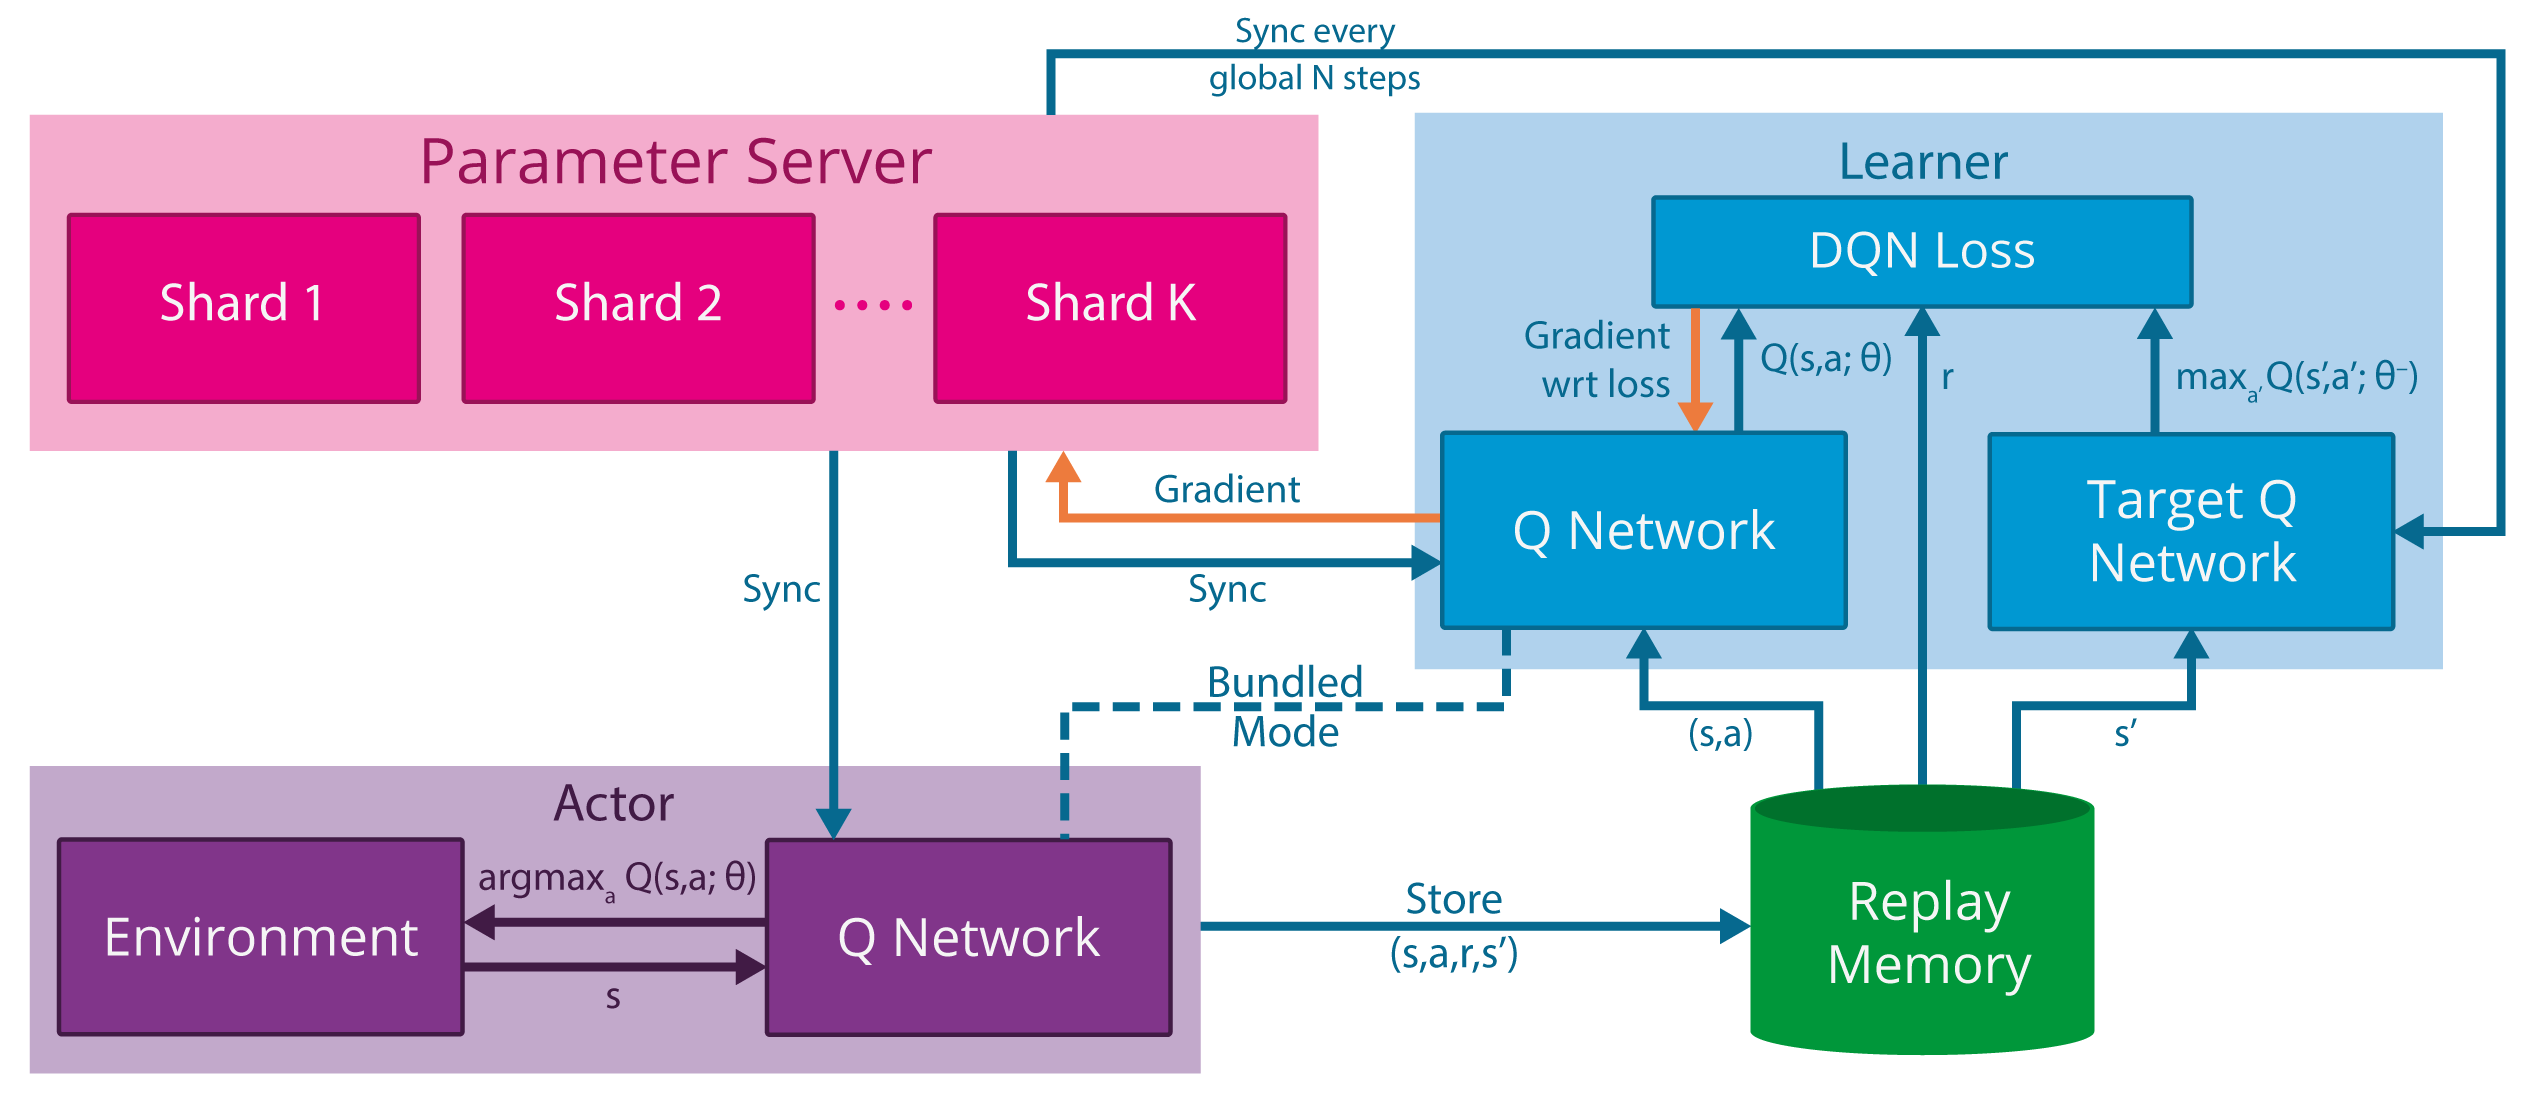
\includegraphics[width=\textwidth]{GorilaArchitecture2c}}
		\caption{The Gorila agent parallelises the training procedure by separating out learners, actors and parameter server. In a single experiment, several learner processes exist and they continuously send the gradients to parameter server and receive updated parameters. At the same time, independent actors can also in parallel accumulate experience and update their Q-networks from the parameter server. }
		\label{Gorila-figure}
	\end{center}
	\vskip -0.2in
\end{figure*}

\begin{algorithm}[t]
	\caption{Distributed DQN Algorithm}
	\label{alg:DistDQNAlgo}
	\begin{algorithmic}
		\STATE Initialise replay memory $D$ to size $P$.
		\STATE Initialise the training network for the action-value function $Q(s,a;\theta)$ with weights $\theta$ and target network $Q(s,a;\theta^-)$ with weights $\theta^- = \theta$.
		\FOR{$episode=1$ {\bfseries to} $M$}
		\STATE Initialise the start state to $s_{1}$.
		\STATE Update $\theta$ from parameters $\theta^+$ of the parameter server.
		\FOR{$t=1$ {\bfseries to} $T$}
		\STATE With probability $\epsilon$ take a random action $a_{t}$ or else $a_{t}$ = $\argmax{a}{Q(s, a ;\theta)}$.
		\STATE Execute the action in the environment and observe the reward $r_t$ and the next state $s_{t+1}$. Store $(s_t,a_t,r_t,s_{t+1})$ in $D$.
		\STATE Update $\theta$ from parameters $\theta^+$ of the parameter server.
		\STATE Sample random mini-batch from $D$. And for each tuple $(s_i,a_i,r_i,s_{i+1})$ set target $y_t$ as
		\IF{$s_{i+1} $ is $terminal$} 
		\STATE $y_t = r_i$
		\ELSE
		\STATE $y_t = r_i + \gamma \max{a'}{Q(s_{i+1}, a' ; \theta^{-})}$
		\ENDIF
		\STATE Calculate the loss $L_t = (y_t - Q(s_i, a_i ; \theta)^2)$.
		\STATE Compute gradients with respect to the network parameters $\theta$ using equation~\ref{eqn:dqngrad}.
		\STATE Send gradients to the parameter server.
		\STATE Every global $N$ steps sync $\theta^{-}$ with parameters $\theta^+$ from the parameter server.
		\ENDFOR
		\ENDFOR
	\end{algorithmic}
\end{algorithm}

We now introduce \emph{Gorila} (General Reinforcement Learning Architecture), a framework for massively distributed reinforcement learning. The Gorila architecture, shown in Figure~\ref{Gorila-figure} contains the following components:

{\bf Actors}. Any reinforcement learning agent must ultimately select actions $a_t$ to apply in its environment. We refer to this process as \emph{acting}. The Gorila architecture contains $N_{act}$ different actor processes, applied to $N_{act}$ corresponding instantiations of the same environment. Each actor $i$ generates its own trajectories of experience $s^i_1, a^i_1, r^i_1, ..., s^i_T, a^i_T, r^i_T$ within the environment, and as a result each actor may visit different parts of the state space. The quantity of experience that is generated by the actors after $T$ time-steps is approximately $TN_{act}$. Each actor contains a replica of the Q-network, which is used to determine behavior, for example using an $\epsilon$-greedy policy. The parameters of the Q-network are synchronized periodically from the parameter server.

{\bf Experience replay memory}. The experience tuples $e^i_t = (s^i_t, a^i_t, r^i_t, s^i_{t+1})$ generated by the actors are stored in a replay memory $D$. We consider two forms of experience replay memory. First, a \emph{local} replay memory stores each actor's experience $D^i_t =  \{ e^i_1, ..., e^i_t \}$ locally on that actor's machine. If a single machine has sufficient memory to store $M$ experience tuples, then the overall memory capacity becomes $MN_{act}$. Second, a \emph{global} replay memory aggregates the experience into a distributed database. In this approach the overall memory capacity is independent of $N_{act}$ and may be scaled as desired, at the cost of additional communication overhead.

{\bf Learners}. Gorila contains $N_{learn}$ learner processes. Each learner contains a replica of the Q-network and its job is to compute desired changes to the parameters of the Q-network. For each learner update $k$, a minibatch of experience tuples $e = (s,a,r,s')$ is sampled from either a local or global experience replay memory $D$ (see above). The learner applies an off-policy RL algorithm such as DQN \cite{mnih2013atari} to this minibatch of experience, in order to generate a gradient vector $g_i$.\footnote{The experience in the replay memory is generated by old behavior policies which are most likely different to the current behavior of the agent; therefore all updates must be performed off-policy \cite{sutton:book}.} The gradients $g_i$ are communicated to the parameter server; and the parameters of the Q-network are updated periodically from the parameter server. 

{\bf Parameter server}. Like DistBelief, the Gorila architecture uses a central parameter server to maintain a distributed representation of the Q-network $Q(s,a; \theta^+)$. The parameter vector $\theta^+$ is split disjointly across $N_{param}$ different machines. Each machine is responsible for applying gradient updates to a subset of the parameters. The parameter server receives gradients from the learners, and applies these gradients to modify the parameter vector $\theta^+$, using an asynchronous stochastic gradient descent algorithm. 

The Gorila architecture provides considerable flexibility in the number of ways an RL agent may be parallelized. It is possible to have parallel acting to generate large quantities of data into a global replay database, and then process that data with a single serial learner. In contrast, it is possible to have a single actor generating data into a local replay memory, and then have multiple learners process this data in parallel to learn as effectively as possible from this experience. However, to avoid any individual component from becoming a bottleneck, the Gorila architecture in general allows for arbitrary numbers of actors, learners, and parameter servers to both generate data, learn from that data, and update the model in a scalable and fully distributed fashion.

The simplest overall instantiation of Gorila, which we consider in our subsequent experiments, is the \emph{bundled} mode in which there is a one-to-one correspondence between actors, replay memory, and learners ($N_{act} = N_{learn}$). Each bundle has an actor generating experience, a local replay memory to store that experience, and a learner that updates parameters based on samples of experience from the local replay memory. The only communication between bundles is via parameters: the learners communicate their gradients to the parameter server; and the Q-networks in the actors and learners are periodically synchronized to the parameter server.

\subsection{Gorila DQN}

We now consider a specific instantiation of the Gorila architecture implementing the DQN algorithm.
As described in the previous section, the DQN algorithm utilizes two copies of the Q-network: a current Q-network with parameters $\theta$ and a target Q-network with parameters $\theta^-$.
The DQN algorithm is extended to the distributed implementation in Gorila as follows.
The parameter server maintains the current parameters $\theta^+$ and the actors and learners contain replicas of the current Q-network $Q(s,a;\theta)$ that are synchronized from the parameter server before every acting step.

The learner additionally maintains the target Q-network $Q(s,a;\theta^-)$.
The learner's target network is updated from the parameter server $\theta^+$ after every $N$ gradient updates in the central parameter server.

Note that $N$ is a global parameter that counts the total number of updates to the central parameter server rather than counting the updates from the local learner.

The learners generate gradients using the DQN gradient given in Equation~\ref{eqn:dqngrad}. However, the gradients are not applied directly, but instead communicated to the parameter server. The parameter server then applies the updates that are accumulated from many learners.

\subsection{Stability}
While the DQN training algorithm was designed to ensure stability of training neural networks with reinforcement learning, training using a large cluster of machines running multiple other tasks poses additional challenges.
The Gorila DQN implementation uses additional safeguards to ensure stability in the presence of disappearing nodes, slowdowns in network traffic, and slowdowns of individual machines.
One such safeguard is a parameter that determines the maximum time delay between the local parameters $\theta$ (the gradients $g_i$ are computed using $\theta$) and the parameters $\theta^+$ in the parameter server.

All gradients older than the threshold are discarded by the parameter server.  Additionally, each actor/learner keeps a running average and standard deviation of the absolute DQN loss for the data it sees and discards gradients with absolute loss higher than the mean plus several standard deviations.  Finally, we used the AdaGrad update rule ~\cite{duchi2011adaptive}.


